\section{Distinction as Search Algorithm}

Given the value that eigenvector-style centrality measures have had in underpinning the logic of internet search algorithms \citep{kleinberg99, brin_page98, langville2005survey-572}, the application of distinction centrality to a reference network is briefly considered. As the social logic of distinction centrality involves jointly considering the interaction between status and constraint, in a reference network the distinction measure will give greater priority to the uniqueness of a node's flow of affiliations. 

A toy reference network is presented in Figure 3. The network was designed to contrast status and distinction within a graph, featuring a clear cluster of nodes with high density and tenuously connected to a node with a high degree of popularity external to the main, denser cluster. Such a graph is supposed to represent a contrast between an orthodox set of mutual endorsements and the emergence of a heterodox set of connections.

The resulting distinction scores are presented in Table 6. The results are ranked from highest to lowest scaled distinction centrality. Node 8 ranks highest in both scaled distinction and status, but immediately afterward, Node 9 and Node 6 switch places in the ordering. Node 6 has the second-highest status, but the third-highest scaled distinction, while Node 9 goes from third in status to second in scaled distinction. The measure rewards the independent connections Node 9 has with Nodes 13 and 14 over the heavier constraints imposed on Node 6. \footnote{In the absence of Node 8's and its constraint effect on Node 6, Node 6 would become the most distinct and highest status.} Node 10's relative position in the social hierarchy is consistent at fourth in both the status and scaled distinction measures.

\begin{figure}
    \captionsetup[subfigure]{font=footnotesize,labelfont=footnotesize}
    \centering
     \begin{subfigure}[b]{0.45\textwidth}
        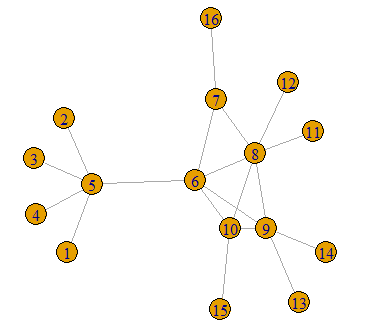
\includegraphics[width=1.0\textwidth]{Plots/search.png}
            \caption{Reference Network Example}
            \label{fig:search-sub}
    \end{subfigure}
    \caption{Example of a non-directed network of references, e.g. citation network, internet links, etc.}
    \label{fig:search-main}
\end{figure}

\input{Tabs/search}

The heterodoxy of Node 5 is elevated to the fifth position in the scaled distinction hierarchy, compared to the sixth position it holds in the status hierarchy. Node 7 correspondingly falls into the sixth position of the scaled distinction hierarchy from the fifth position in terms of status. However, scaled distinction centrality also elevates Nodes 1, 2, 3, and 4, which buttress 5's popularity. These nodes have the lowest status, yet leap over the hangers onto the core members of the main orthodox cluster. They are greatly penalized for their high level of constraint, whereas Node's 1, 2, 3, and 4 are empowered by 5's own lower status position. If the goal is to elevate uniqueness, this makes sense, as Nodes 11 through 16 are likely to conform to their higher-status, high-distinction connections. Nodes 7, 8, 9, and 10 already implicitly represent their contributions. Additionally, the application of the scalar is important in the final results. Without the scalar, Node 5 would actually be the third-ranked node in terms of distinction, leaping Node 6. Such a result may be desirable in technical applications where uniqueness should be privileged over social hierarchy. On the whole, the scaled distinction centrality measure helps highlight a node's uniqueness in search applications. 